We present a summary of the difference in treatment effects between males and females. For each outcome, $Y$, we estimate  Equation~\eqref{eq:te}, which accounts for the levels of the treatment effect and the ``male'' effect,

\begin{equation}
\label{eq:te}
Y = \beta_0 + \beta_1 [\text{treatment}] + \beta_2 [\text{male}] + \beta_3 [\text{treatment} \times \text{male}] + \beta X + \varepsilon.
\end{equation}

\noindent Assuming that $\varepsilon$ is a mean-zero and conditionally independent disturbance, the estimated $\beta_3$ reveals the gender difference of the treatment effect.

We group the outcomes by broad, life-relevant categories and code the outcomes such that $\beta_1 > 0$ indicates a more socially positive treatment effect. We resample with replacement 100 times. In each bootstrap, we calculate, by category, the proportion of variables for which the gender differences ($\beta_3$) is negative. A negative gender difference indicates that the treatment has a more socially positive effect on females than on males after controlling for the treatment effect, the male effect, and background variables unaffected by treatment.\footnote{These background variables are mother's IQ and mother's years of education when the subject was born.}

As seen in Appendix~\ref{app:data}, measures of IQ and achievement are internally consistent within and across time periods. This is not always the case for social-emotional skills. We leverage the consistency of the cognitive measures to create additional measures of achievement net of IQ. This captures the skill measured by achievement scores orthogonal to that measured by IQ scores.

Figure~\ref{fig:prop-category} shows, for each category, the proportion of variables with negative gender differences ($\beta_3 < 0$, females $>$ males). When aggregating all outcomes, the gender differences are not apparent: 54.2\% of all gender differences are negative, but this is not statistically different from the null hypothesis of 50\%. However, dividing the variables by category shows considerable gender differences. Females have more positive effects on achievement and social-emotional scores, using both traditional social-emotional batteries and the social-emotional construct described above. Treatment also more positively affected them when considering labor market outcomes (including education, employment, and income) and crime outcomes. Consistent with other studies, males benefit more in health outcomes.\footnote{\citet{Campbell_Conti_etal_2014_EarlyChildhoodInvestments,Conti_etal_2016_LongTermHealth}.}

\begin{figure}[H]
\begin{center}
\caption{Proportion of Outcomes with Negative Gender Difference by Category}
\label{fig:prop-category}
\includegraphics[width=\textwidth]{../output/abccare-counts-category}
\end{center}
\raggedright \footnotesize
Note: Each category is comprised of related variables. All variables are coded such that higher values correspond to socially positive outcomes. Teen Ach. net IQ is achievement at ages 12 and 15 net of IQ. Late Ach. net IQ is the same but for achievement at age 21. Labor and Parent include education, employment, and income variables for the subject and parent, respectively. 
\end{figure}

\begin{table}[H]
\centering
\caption{Treatment Effects, Parenting Skills}
\label{te-parenting}
\begin{adjustbox}{width=\textwidth}
\begin{threeparttable}
	\input{../output/abccare-parenting}
\begin{tablenotes}
\item Note: This table displays the treatment effects 
\end{tablenotes}
\end{threeparttable}
\end{adjustbox}
\end{table}

\begin{table}[H]
\centering
\caption{Treatment Effects, Cognitive Skills}
\label{te-cognitive}
\begin{adjustbox}{width=\textwidth}
\begin{threeparttable}
	\input{../output/abccare-cognitive}
\begin{tablenotes}
\item Note:
\end{tablenotes}
\end{threeparttable}
\end{adjustbox}
\end{table}

\begin{table}[H]
\centering
\caption{Treatment Effects, Non-cognitive Skills}
\label{te-ncognitive}
\begin{adjustbox}{width=\textwidth}
\begin{threeparttable}
	\input{../output/abccare-ncognitive}
\begin{tablenotes}
\item Note:
\end{tablenotes}
\end{threeparttable}
\end{adjustbox}
\end{table}

\begin{table}[H]
\centering
\caption{Treatment Effects, Education}
\label{te-education}
\begin{adjustbox}{width=\textwidth}
\begin{threeparttable}
	\input{../output/abccare-education}
\begin{tablenotes}
\item Note:
\end{tablenotes}
\end{threeparttable}
\end{adjustbox}
\end{table}


\subsection{Inputs}

We explore the effects of the intervention on parenting in more detail. This allows us to understand the gender differences of this important input. We use measurements of the Home Observation for Measurement of the Environment (HOME; \citet{Bradley-Caldwell_1977_AJMD}), which measures the quality of the child's home environment.\footnote{Although the exact scales vary by age, the subscales of the HOME measure generally measure maternal warmth and involvement, absence of punishment, provision of appropriate toys, encouragement of mature behavior and independence, and the physical and language environment. The full score is the sum of these subscales.}

When graphing the density of a factor combining the full HOME scores measured at different ages, the density of the treatment group in both the male and female subsamples is bimodal (Figure~\ref{fig:total-home}). Because this is not the case for the control group, it is possible that treatment is moderated by another input of home environment. We consider the input of father's presence. For males, the mean of the treatment group if the father is present is greater than that of the treatment group if the father is absent. The reverse is seen for the females. 

\begin{figure}
\begin{center}
\caption{Density of the HOME Scores by Gender and Experimental Group}
\label{fig:total-home}

	\begin{subfigure}[b]{0.49\textwidth}
		\centering
		\caption{Factor HOME Scores, Males}
		\label{fig:home-male-factor}
			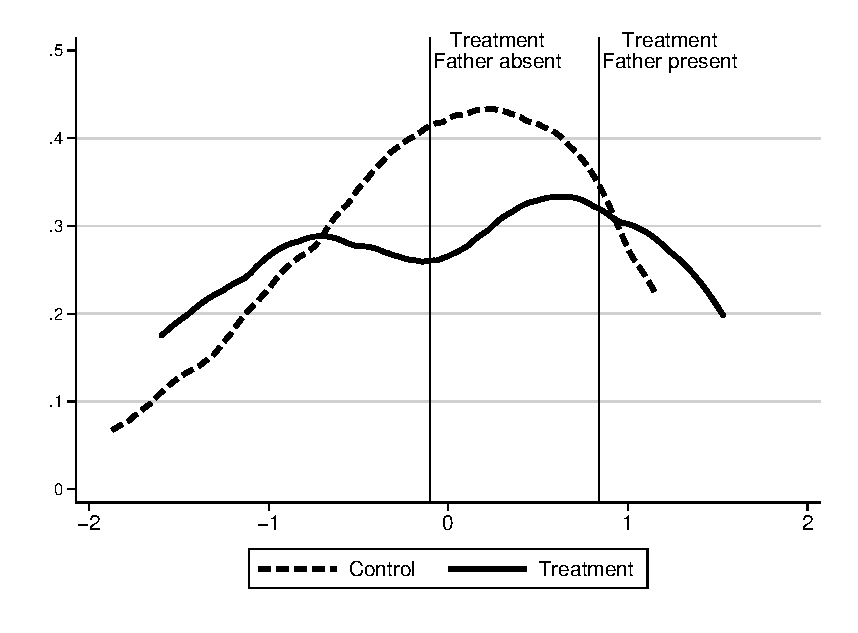
\includegraphics[width=\textwidth]{../output/HOME-males-factorhome}
	\end{subfigure}
	\begin{subfigure}[b]{0.49\textwidth}
		\centering
		\caption{Factor HOME Scores, Females}
		\label{fig:home-female-factor}
			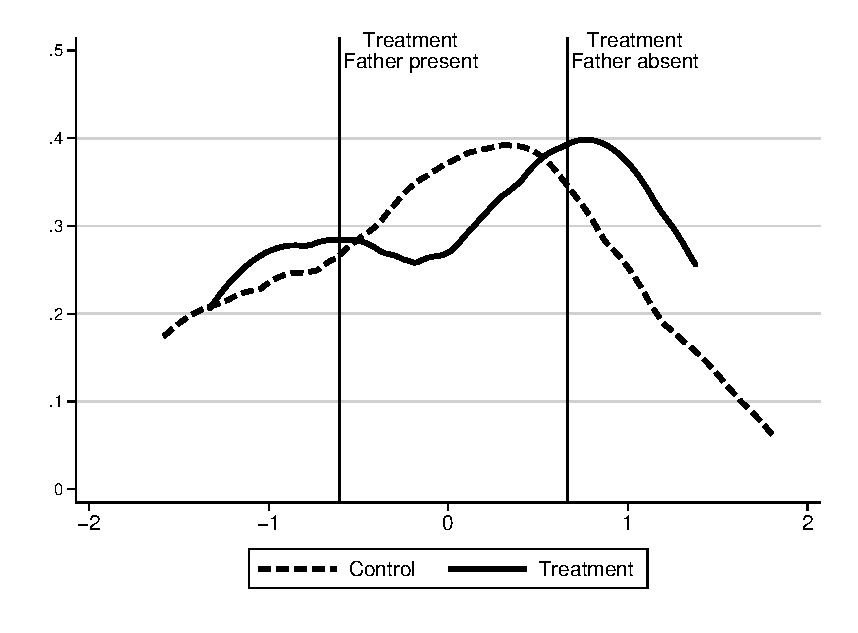
\includegraphics[width=\textwidth]{../output/HOME-females-factorhome}
	\end{subfigure}
\end{center}
\raggedright
Note: These plots show the distribution the factor of HOME scores. The factors are computed by gender using full HOME scores at 0.5, 1.5, 2.5, and 8 years. The vertical lines are the means of the treatment group by father's presence. 
\end{figure}

We explore this trend more closely in Figure~\ref{fig:total-home-quantiles}. To do so, we calculate the distribution pooling experimental groups but splitting by gender and father's presence. We then calculate, by gender and father's presence, the proportion of the treatment group that is in quantile 1 versus quantile 2. We do the same for the control group. 

The result of this exercise shows that the bimodal shape of the densities of the treatment group is explained differently by gender. For males, the HOME scores are higher for the control group when the fathers are absent and higher for the treatment group when father's are present. For females, the opposite is the case: The HOME scores are higher for the control group when fathers are present and higher for the treatment group when fathers are absent. 

One explanation of this is that treatment complements father's presence for males but substitutes it for females. Mothers then compensate for the father's absence for males (females) in the control (treatment) group. 

%One way mothers can compensate for the father's absence for males is to enroll them in alternate preschool arrangements. This is seen with more males in the control group being enrolled in these arrangements than control-group females (Figure~\ref{fig:alt-enrollment}). 

\begin{sidewaysfigure}
\begin{center}
\caption{Factor HOME Scores}
\label{fig:total-home-quantiles}
	\begin{subfigure}[b]{0.49\textwidth}
		\centering
		\caption{HOME, Father Absent, Males}
		\label{fig:home-male-mean}
			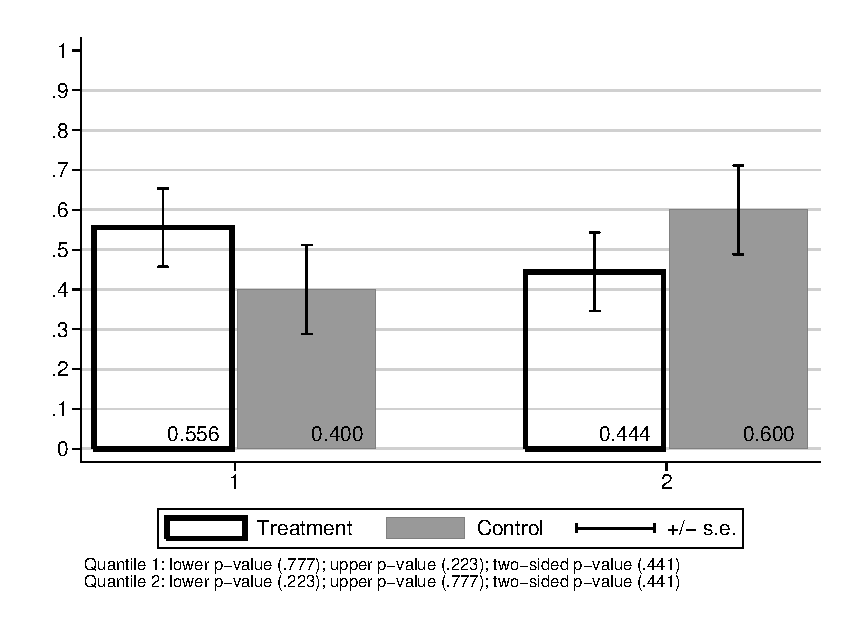
\includegraphics[width=\textwidth]{../output/HOME-male1-fhome0-2quant}
	\end{subfigure}
	\begin{subfigure}[b]{0.49\textwidth}
		\centering
		\caption{HOME, Father Absent, Females}
		\label{fig:home-female-mean}
			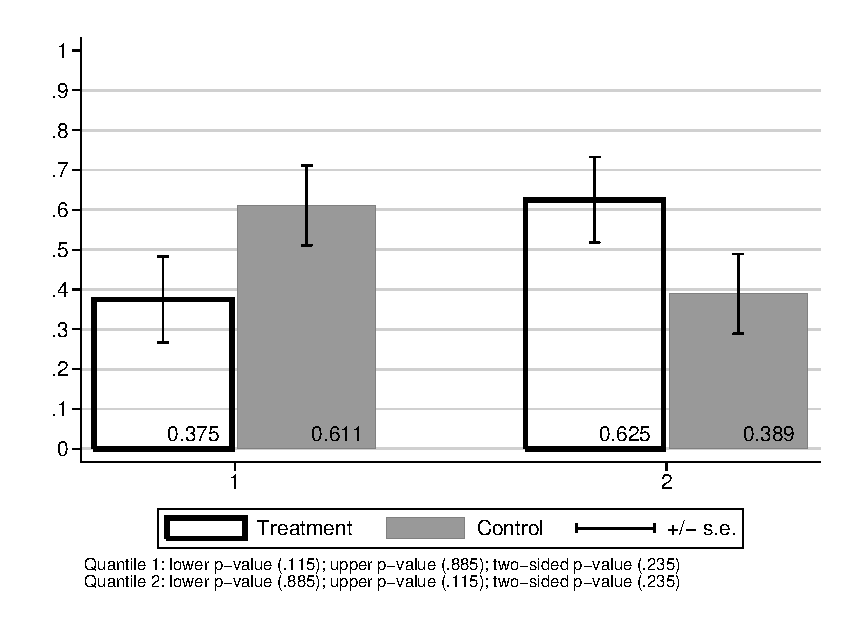
\includegraphics[width=\textwidth]{../output/HOME-male0-fhome0-2quant}
	\end{subfigure}
	
	\begin{subfigure}[b]{0.49\textwidth}
		\centering
		\caption{HOME, Father Present, Males}
		\label{fig:home-male-factor}
			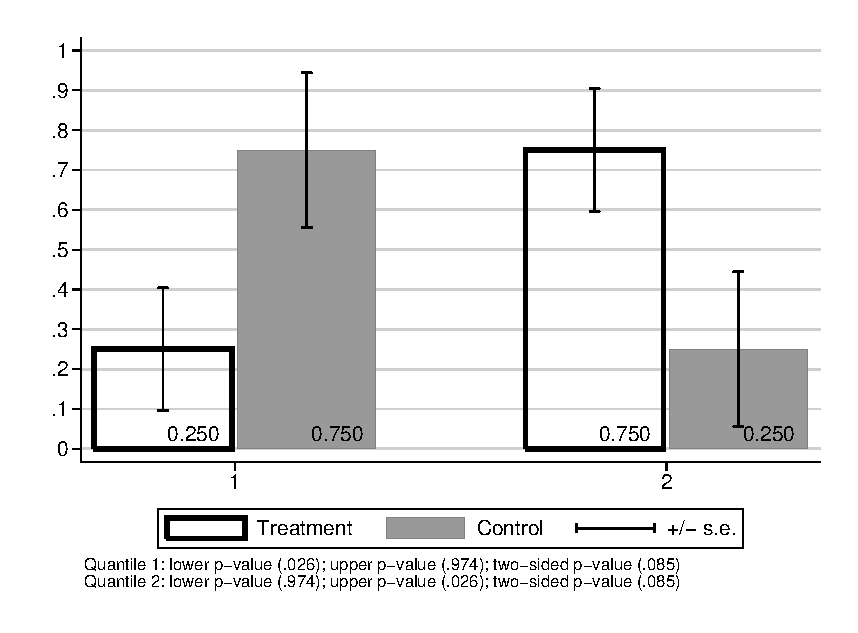
\includegraphics[width=\textwidth]{../output/HOME-male1-fhome1-2quant}
	\end{subfigure}
	\begin{subfigure}[b]{0.49\textwidth}
		\centering
		\caption{HOME, Father Present, Females}
		\label{fig:home-female-factor}
			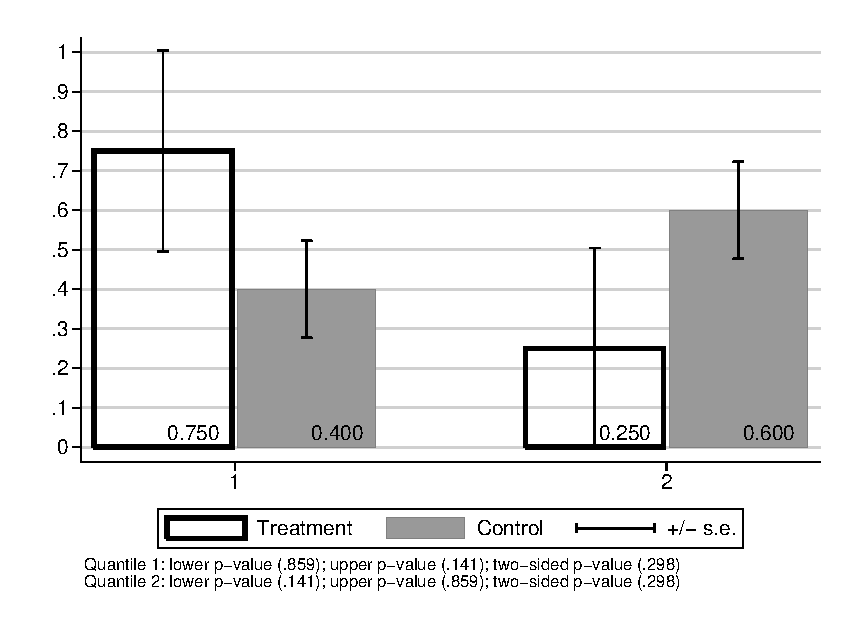
\includegraphics[width=\textwidth]{../output/HOME-male0-fhome1-2quant}
	\end{subfigure}
\end{center}
\raggedright \footnotesize
Note: The horizontal axis divides a factor of the HOME scores into the first and second quantile of the distribution pooling across experimental groups, but splitting  by gender and father's presence. The factors are computed by gender using full HOME scores at 0.5, 1.5, 2.5, and 8 years. The lower $p$-value tests that the treatment proportion is less than the control proportion within a quantile. The upper $p$-value tests that the treatment proportion is greater than the control proportion within a quantile. The numbers reported in the bars are the proportions. All standard errors and $p$-values are calculated using 1,000 bootstraps.
\end{sidewaysfigure}

%\begin{figure}
%\begin{center}
%\caption{Alternate Preschool Enrollment}
%\label{fig:alt-enrollment}
%	\begin{subfigure}[b]{0.49\textwidth}
%		\centering
%		\caption{Males by Father's Presence}
%			\includegraphics[width=\textwidth]{../output/family-dcmopre-father-male}
%	\end{subfigure}
%	\begin{subfigure}[b]{0.49\textwidth}
%		\centering
%		\caption{Females by Father's Presence}
%			\includegraphics[width=\textwidth]{../output/family-dcmopre-father-female}
%	\end{subfigure}
%	
%		\begin{subfigure}[b]{0.49\textwidth}
%		\centering
%		\caption{Pooled}
%			\includegraphics[width=\textwidth]{../output/family-dcmopre}
%	\end{subfigure}
%	\end{center}
%\raggedright
%Note: These histograms display the distributions of the months of enrollment in alternative preschool by gender. Months of enrollment are cumulative between birth and 5 years. 
%\end{figure}

\subsection{Adult Outcomes}

\begin{figure}[H]
\begin{center}
\caption{Crime}
\label{fig:}	
	\begin{subfigure}[b]{0.49\textwidth}
		\centering
		\caption{Felonies}
			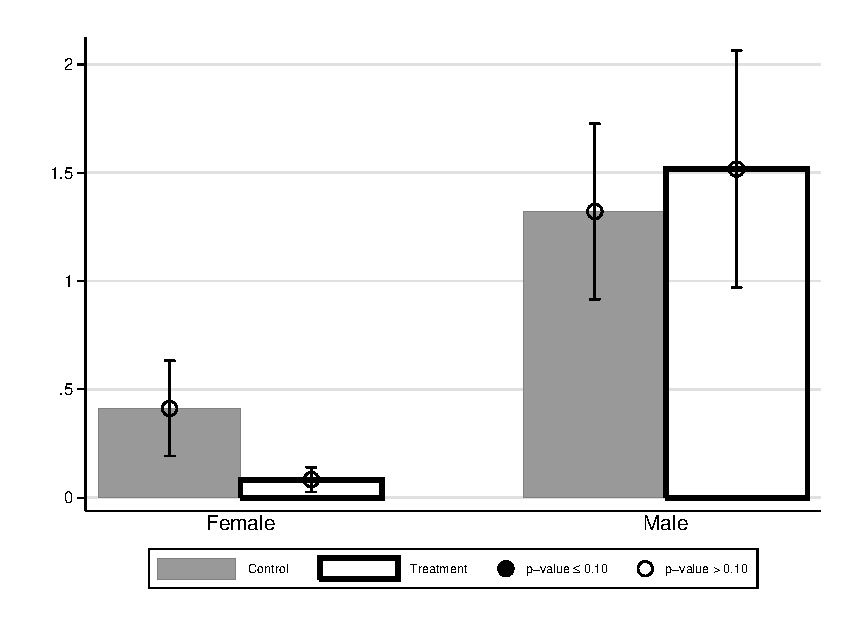
\includegraphics[width=\textwidth]{../output/Outcomes_Correlation/abccare/crime/bar-gender-trt-ad34_fel}
		\end{subfigure}
	\begin{subfigure}[b]{0.49\textwidth}
		\centering
		\caption{Misdemeanors}
			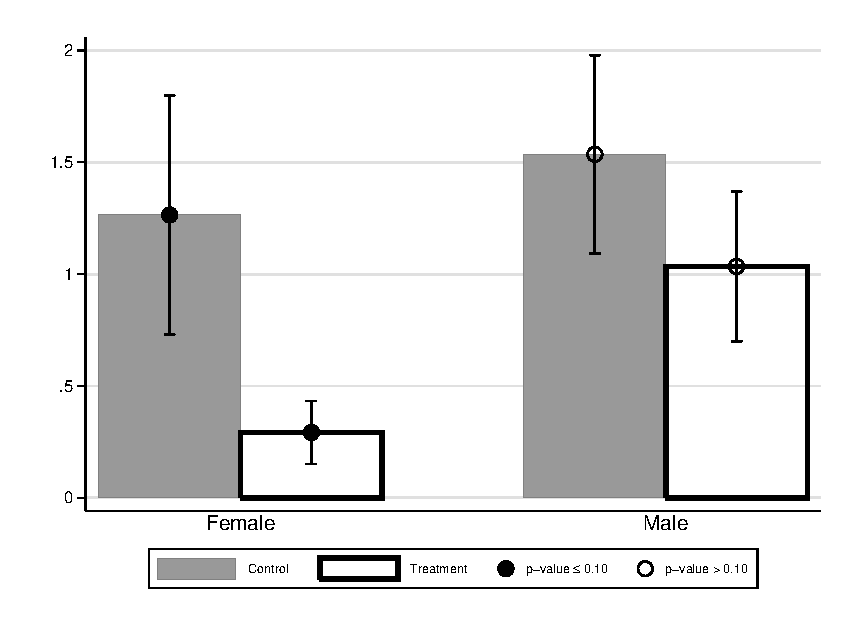
\includegraphics[width=\textwidth]{../output/Outcomes_Correlation/abccare/crime/bar-gender-trt-ad34_mis}
	\end{subfigure}
	\end{center}
\raggedright \footnotesize
Note:
\end{figure}

\begin{figure}[H]
\begin{center}
\caption{Age of First Crime}
\label{fig:age-first-crime}
	\includegraphics[width=\textwidth]{../output/Outcomes_Correlation/abccare/crime/bar-gender-trt-juv_crime_age}
\end{center}
\raggedright \footnotesize
Note:
\end{figure}